\documentclass{beamer}

\mode<presentation>
{
  \usetheme{Pittsburgh}
  \useoutertheme{split}
  \setbeamercovered{transparent} 
  \setbeamertemplate{navigation symbols}{}
  \setbeamertemplate{title}{}
  % \setbeamertemplate{footline}[page number]{}
  % \setbeamertemplate{footline}[frame number]
}

\usepackage{amsmath}
\usepackage[english]{babel}
\usepackage[utf8]{inputenc}
\usepackage{times}
\usepackage[T1]{fontenc}
\usepackage{graphicx}
\usepackage{hyperref}
\usepackage{subfigure}
\usepackage{setspace}
\usepackage{multirow}
\usepackage{booktabs}
\usepackage{tabulary}
\usepackage{tabu}
\usepackage{verbatim}

\title[Flow Control, Functions]
{Flow Control, Functions, and Scientific Computing}

\author{INF1005/6 - Social Data Analytics}
\institute[] {
    Professor Alex Hanna
}

\date[] {
January 19, 2017
}

\begin{document}

\begin{frame}
  \titlepage
\end{frame}

\begin{frame}{Flow Control}
    \begin{columns}
        \begin{column}{0.5\textwidth}
            Flow control refers which parts of the program are executed, in what order. \\
            \vspace*{1em}
            Types of flow control
            \begin{itemize}[<2->]
                \item Loops
                \item Conditional statements
                \item Functions
            \end{itemize}
        \end{column}
        \begin{column}{0.4\textwidth}
            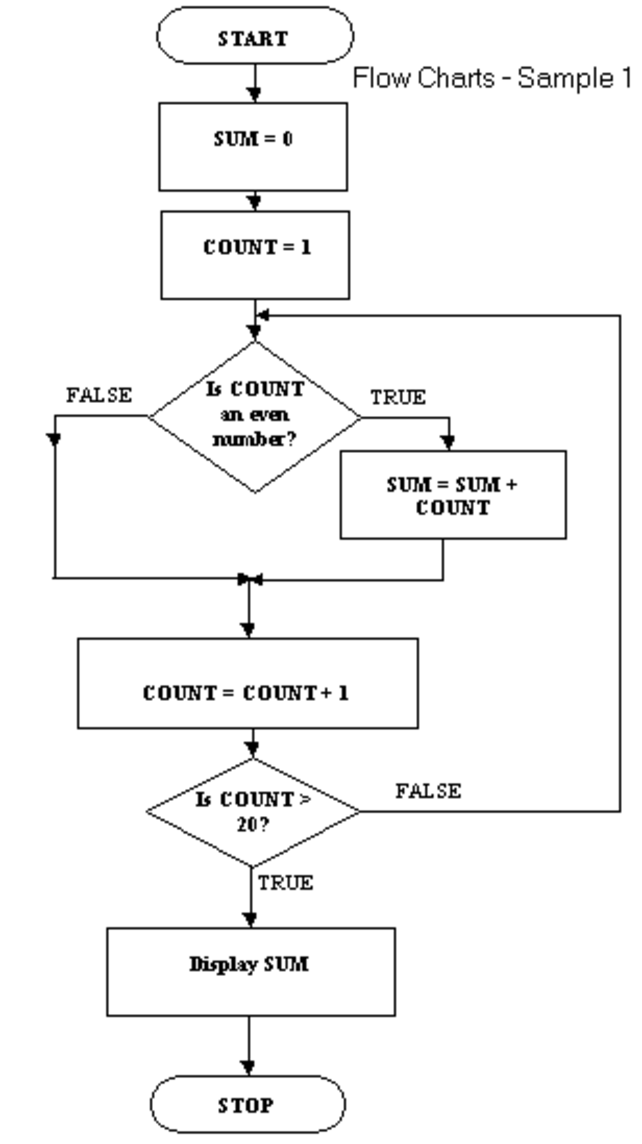
\includegraphics[width=0.9\textwidth]{img/flow-chart.pdf}
        \end{column}
    \end{columns}
\end{frame}

\begin{frame}[fragile]{Loops}
\texttt{for} loop
\begin{verbatim}

    for i in range(100):
        print(i)
\end{verbatim}
\end{frame}

\begin{frame}[fragile]{Loops}
\texttt{while} loop
\begin{verbatim}

    i = 0
    while i < 100:
        print(i)
        i = i + 1
\end{verbatim}
\end{frame}

\begin{frame}[fragile]{Conditional statements}
    \begin{columns}
        \begin{column}{0.5\textwidth}
            \textbf{if} it is raining then \\ 
            the sky is cloudy \\
            \textbf{else if} it is snowing then \\
            the sky is cloudy \\
            \textbf{else} \\
            the sky is clear
        \end{column}
        \begin{column}{0.5\textwidth}
\begin{block}<2>{}
\footnotesize
\begin{verbatim}

    sky = None
    is_raining = True
    is_snowing = False
    if is_raining:
        sky = "cloudy"
    elif is_snowing:
        sky = "cloudy"
    else:
        sky = "clear"
\end{verbatim}
\end{block}
        \end{column}
    \end{columns}
\end{frame}

\begin{frame}[fragile]{Conditional statements}
    \begin{columns}
        \begin{column}{0.5\textwidth}
            \textbf{if} it is raining then \\ 
            the sky is cloudy \\
            \textbf{else if} it is snowing then \\
            the sky is cloudy \\
            \textbf{else} \\
            the sky is clear \\
            \vspace*{1em}
            \texttt{is\_raining} and \texttt{is\_snowing} are booleans
        \end{column}
        \begin{column}{0.5\textwidth}
\begin{block}{}
\footnotesize
\begin{verbatim}

    sky = None
    is_raining = True
    is_snowing = False
    if is_raining == True:
        sky = "cloudy"
    elif is_snowing == True:
        sky = "cloudy"
    else:
        sky = "clear"
\end{verbatim}
\end{block}
        \end{column}
    \end{columns}
\end{frame}

\begin{frame}[fragile]{Comparison Operators}
    \begin{columns}
        \begin{column}{0.5\textwidth}
            Numerical operators
            \begin{itemize}[<+->]
                \item \texttt{==}
                \item \texttt{!=}
                \item \texttt{>}
                \item \texttt{>=}
                \item \texttt{<}
                \item \texttt{<=}
            \end{itemize}
        \end{column}
        \begin{column}{0.5\textwidth}
        \begin{block}<7>{}
        Examples
\begin{verbatim}

    3 == 4 # False 
    3 != 4 # True 
    3 > 4  # False 
    3 < 4  # True 
\end{verbatim}
        \end{block}
        \end{column}
    \end{columns}
\end{frame}

\begin{frame}[fragile]{Logical Operators}
    \begin{columns}
        \begin{column}{0.4\textwidth}
            Logical operators tie various logical statements together
            \begin{itemize}
                \item \texttt{and}
                \item \texttt{or}
            \end{itemize}
        \end{column}
        \begin{column}{0.6\textwidth}
        \small
\begin{verbatim}

    True and True
    True and False
    False and False
    True or True
    True or False
    False or False
\end{verbatim}
        \end{column}
    \end{columns}
\end{frame}

\begin{frame}[fragile]{Logical Operators}
    \begin{columns}
        \begin{column}{0.4\textwidth}
            Logical operators tie various logical statements together
            \begin{itemize}
                \item \texttt{and}
                \item \texttt{or}
            \end{itemize}
        \end{column}
        \begin{column}{0.6\textwidth}
        \small
\begin{verbatim}

    True and True    # True
    True and False   # False
    False and False  # False
    True or True     # True
    True or False    # True
    False or False   # False
\end{verbatim}
        \end{column}
    \end{columns}
\end{frame}

\begin{frame}[fragile]{Logical Operators}
You can combine logical operations with operators
\begin{verbatim}

    (4 > 3) and (8 > 5)            # True
    True or (0.2 < -2)             # True
    (-3 == 2) and (3 == 3)         # False
    ("hello" == "kitty") and True  # False
\end{verbatim}

\begin{block}{}<2>
You can also assign them to variables
\begin{verbatim}

    is_4gt3 = 4 > 3
    is_8gt5 = 8 > 5
    is_4gt3 and is_8gt5 # True
\end{verbatim}
\end{block}
\end{frame}

\begin{frame}[fragile]{Using Conditional Statements}
    \begin{columns}
        \begin{column}{0.3\textwidth}
            \texttt{if}, \texttt{elif}, and \texttt{while} all work with a conditional statement
        \end{column}
        \begin{column}{0.7\textwidth}
        \footnotesize

\begin{block}{}<2->
\begin{verbatim}
    import random
    count = random.randint(-10, 10)
    if count < 0:
        print("count is negative.")
    elif count == 0:
        print("count is zero.")
    else: 
        print("count is positive.")
\end{verbatim}
\end{block}
\vspace*{-1em}
\begin{block}{}<3->
\begin{verbatim}
    count = -10
    while count < 0:
        print("count is negative")
        print(count)
        count = random.randint(-10, 10)
\end{verbatim}
\end{block}
        \end{column}
    \end{columns}
\end{frame}

\begin{frame}{Exercises}
    \begin{enumerate}
        \item Write code which goes through each number from 0 to 20 and prints the number if it is divisible by 5.
        \item Write code which begins with a number equal to 1000. Print the number, then subtract 1 from the variable until the number equals zero. 
    \end{enumerate}
\end{frame}

\begin{frame}{Functions}
    \begin{itemize}[<+->]
        \item A \textit{function} is a piece of code which can be written once and run many times
        \item Examples of built-in functions: \texttt{range}, \texttt{print}, \texttt{randint}
        \item Two most important parts of a function
            \begin{itemize}
                \item \textit{arguments} - what goes between the parentheses
                \item \textit{return value} - what comes back
                \item Both are optional
            \end{itemize}
    \end{itemize}
\end{frame}

\begin{frame}[fragile]{Built-in Functions}
    \begin{columns}
        \begin{column}{0.5\textwidth}
            List functions
            \begin{itemize}[<+->]
                \item \texttt{len} - length of list
                \item \texttt{sorted} - sorts a list
                \item \texttt{list} - converts to list 
            \end{itemize}
        \end{column}
        \begin{column}{0.5\textwidth}
        \small
\begin{block}{}
\begin{verbatim}
    len([1, 2, 3])
    # 3
\end{verbatim}
\end{block}
\vspace*{-1em}
\begin{block}<2->{}
\begin{verbatim}
    sorted([3, 2, 1])
    # [1, 2, 3]
\end{verbatim}
\end{block}
\begin{block}<3->{}
\vspace*{-1em}
\begin{verbatim}
    list( (1, 2, 3) )
    # [1, 2, 3]
\end{verbatim}
\end{block}
        \end{column}
    \end{columns}
\end{frame}

\begin{frame}[fragile]{Built-in Functions}
    \begin{columns}
        \begin{column}{0.5\textwidth}
            Type functions
            \begin{itemize}[<+->]
                \item \texttt{type} - get type of object
                \item \texttt{int} - convert to integer
                \item \texttt{float} - convert to float
                \item \texttt{str} - convert to string
            \end{itemize}
        \end{column}
        \begin{column}{0.5\textwidth}
        \small
\begin{block}{}
\begin{verbatim}
    type([1, 2, 3])
    # list

    type(1.3)
    # float
\end{verbatim}
\end{block}
\vspace*{-3em}
\begin{block}<2->{}
\begin{verbatim}
    int("10")
    # 10

    float(1000)
    # 1000.0
\end{verbatim}
\end{block}
\vspace*{-3em}
\begin{block}<4->{}
\begin{verbatim}
    str(100)
    Out[]: '100'
\end{verbatim}
\end{block}
        \end{column}
    \end{columns}
\end{frame}

\begin{frame}[fragile]{User-defined functions}
    \begin{columns}
        \begin{column}{0.3\textwidth}
            Define your own functions if you plan using the same piece of code over and over.
        \end{column}
        \begin{column}{0.7\textwidth}
        \small
\begin{block}{}
\begin{verbatim}
    def my_mean(my_list):
        sum = 0
        for i in my_list:
            sum += i
        return sum / len(my_list)

    my_mean([1, 2, 4, 8, 10])
    # 5.0
\end{verbatim}
\end{block}  
        \end{column}
    \end{columns}
\end{frame}

\begin{frame}[fragile]{User-defined functions}
    \begin{columns}
        \begin{column}{0.3\textwidth}
            \texttt{def} says that this will be a user-defined function.
        \end{column}
        \begin{column}{0.7\textwidth}
        \small
\begin{block}{}
\begin{semiverbatim}
    \textbf{def} my_mean(my_list):
        sum = 0
        for i in my_list:
            sum += i
        return sum / len(my_list)

    my_mean([1, 2, 4, 8, 10])
    # 5.0
\end{semiverbatim}
\end{block}  
        \end{column}
    \end{columns}
\end{frame}

\begin{frame}[fragile]{User-defined functions}
    \begin{columns}
        \begin{column}{0.3\textwidth}
            What comes after \texttt{def} is the function name.
        \end{column}
        \begin{column}{0.7\textwidth}
        \small
\begin{block}{}
\begin{semiverbatim}
    def \textbf{my_mean}(my_list):
        sum = 0
        for i in my_list:
            sum += i
        return sum / len(my_list)

    my_mean([1, 2, 4, 8, 10])
    # 5.0
\end{semiverbatim}
\end{block}  
        \end{column}
    \end{columns}
\end{frame}

\begin{frame}[fragile]{User-defined functions}
    \begin{columns}
        \begin{column}{0.3\textwidth}
            In between the parentheses are the arguments. You use them as variables within the function.
        \end{column}
        \begin{column}{0.7\textwidth}
        \small
\begin{block}{}
\begin{semiverbatim}
    def my_mean(\textbf{my_list}):
        sum = 0
        for i in \textbf{my_list}:
            sum += i
        return sum / len(\textbf{my_list})

    my_mean([1, 2, 4, 8, 10])
    # 5.0
\end{semiverbatim}
\end{block}  
        \end{column}
    \end{columns}
\end{frame}

\begin{frame}[fragile]{User-defined functions}
    \begin{columns}
        \begin{column}{0.3\textwidth}
            \texttt{return} is a special function which gives a value back from the function.
        \end{column}
        \begin{column}{0.7\textwidth}
        \small
\begin{block}{}
\begin{semiverbatim}
    def my_mean(my_list):
        sum = 0
        for i in my_list:
            sum += i
        \textbf{return} sum / len(my_list)

    my_mean([1, 2, 4, 8, 10])
    5.0
\end{semiverbatim}
\end{block}  
        \end{column}
    \end{columns}
\end{frame}


\begin{frame}{Methods}
    A \textit{method} is a function which is associated with an object. The big difference is the syntax, which is
    \begin{center}
        \texttt{object.method(args)}
    \end{center}
\end{frame}

\begin{frame}[fragile]{List methods}
\begin{semiverbatim}
    my_list = [1, 2, 3]
    my_list.append(4)
    \visible<2->{# [1, 2, 3, 4]}

    \visible<3->{my_list.extend([1, 2, 4])}
    \visible<4->{# [1, 2, 3, 4, 1, 2, 4]}

    \visible<5->{my_list.count(4)}
    \visible<6->{# 2}

    \visible<7->{my_list.remove(1)}
    \visible<8->{# [2, 3, 4, 1, 2, 4]}

    \visible<9->{my_list.clear()}
    \visible<10->{# []}
\end{semiverbatim}
\end{frame}

\begin{frame}[fragile]{String methods}
\small
\begin{semiverbatim}
    my_string = "this is a string. it is a good string"
    my_string.capitalize()
    \visible<2->{# 'This is a string. it is a good string'}

    \visible<3->{my_string.find("it")}
    \visible<4->{# 18}

    \visible<5->{my_string.count("is")}
    \visible<6->{# 2}

    \visible<7->{my_string.replace("string", "bit of text")}
    \visible<8->{# 'this is a bit of text. it is a good bit of text'}

    \visible<9->{my_string.split()}
    \visible<10->{# ['this', 'is', 'a', 'string.', 'it', 'is', 
        'a', 'good', 'string']}
\end{semiverbatim}
\end{frame}

\begin{frame}{Exercises}
    \begin{enumerate}
        \item Write a function which checks if a string is in another string. If so, return True. If not, return False.
        \item Write a function which takes two numbers $x$ and $y$, raises $x$ to the $y$ power, and subtracts one, i.e. $f(x, y) = x^y - 1$. Return the result.
    \end{enumerate}
\end{frame}

\begin{frame}{Modules}
    \begin{columns}
        \begin{column}{0.4\textwidth}
            \textit{Modules} are prewritten libraries of objects and functions.
        \end{column}
        \begin{column}{0.6\textwidth}
        Three ways of importing modules
        \small
\begin{block}{}
\begin{semiverbatim}
    \visible<1->{
    import random
    random.randint(-1, 1)
    } 

    \vspace*{0.5em}

    \visible<2->{
    import random as ra
    ra.randint(-1, 1)
    } 

    \vspace*{0.5em}

    \visible<3->{
    from random import randint
    randint(-1, 1)
    } 
\end{semiverbatim}
\end{block}  
        \end{column}
    \end{columns}
\end{frame}

\begin{frame}{SciPy and pandas}
    \begin{columns}
        \begin{column}{0.5\textwidth}
            \textit{SciPy} is a module for scientific and technical computing. \\
            \vspace*{0.5em}
            \textit{pandas} is a module for data manipulation and analysis.
        \end{column}
        \begin{column}{0.5\textwidth}
        \small
        We will usually import these two modules like so: \\
        \vspace*{0.5em}
        \texttt{import numpy as np} \\
        \texttt{import pandas as pd}
        \end{column}
    \end{columns}
\end{frame}

\end{document}
